%	Требования технического задания на разработку СУ ПТДУ
\anonsection{ОСНОВНАЯ ЧАСТЬ}
\section{Требования технического задания на разработку СУ ПТДУ}

\begin{enumerate}
	\item Рассматривается схема газосвязанной ПТДУ с регулированием тяги
	
	\item Основные потребные параметры ПТДУ определяются значениями
	\begin{itemize}
		\item Диапазон суммарной тяги $R_{\sum} = 9.0 - 22.0$ тс, при этом предполагается возможность реализации управления тягой по заданным алгоритмам в зависимости от реализованных условий посадки, обусловленных разбросом параметров атмосферы, аэродинамических, массовых, инерционных, центровочных характеристик возвращаемого аппарат, параметров, траектории и др
		\item Суммарный импульс тяги по осям всех сопел $I_{\sum} = 2745 \  \text{кН} \cdot \text{c}$
		\item Максимальное время работы $30$ c.
	\end{itemize}
	\item Рассматривается применение в составе ПТДУ от 8 до 12 сопловых управляющих блоков (СУБ), Каждый СУБ имеет два расходных сопла, одно из которых направлено вдоль продольной оси ВА, второе-под углом (30… 45) грд к поперечной плоскости ВА. Регулирование расхода через каждое сопло осуществляется по командам от систем управления дифференцированно с помощью регулятора механического типа, вал которого кинематически связан с рулевой машинкой по командам управления.
	
	\item Сопла, направленные вдоль продольной оси ВА (сопла первой группы), задействуются на основном участке торможения от момента начала работы ПТДУ и до высоты 40 м, с которой начинается приземный участок торможения. Группа обеспечивает гашение линейной скорости ВА на этом участке, а также управление относительно ЦМ по каналам рысканья и тангажа.
	
	\item Сопла, направленные под углом (30…45) грд к поперечной плоскости ВА (сопла второй группы), введены в состав ПТДУ для минимизации воздействия струй работающей ПТДУ на грунт. Сопла второй группы задействуются на приземном участке, а также для управления по каналам рысканья и тангажа на основном участке (при необходимости) и на приземном.
	
	\item Должна быть проработана целесообразность и, при необходимости, реализация управления по каналу крена средствами ПТДУ при ее работе.
\end{enumerate}
\clearpage

\subsection{Назначение ПТДУ}
Посадочная твердотопливная двигательная установка (ПТДУ) предназначена для снижения скорости возвращаемого орбитального аппарата (ВА) на участке приземления от величин, соответствующих установившейся скорости спуска, до заданных значений к моменту касания земли. При этом должна обеспечиваться возможность реализации управления тягой по заданным алгоритмам в зависимости от реализованных условий посадки по командам системы управления ВА.	

Под участком приземления понимается участок спуска ВА, начинающийся в момент включения ПТДУ и заканчивающийся в момент касания первой опоры посадочного устройства (ПУ) ВА с поверхностью полигона. Приведение ВА на полигон обеспечивается управлением ВА до включения ПТДУ. Под полигоном понимается подготовленная посадочная площадка диаметром несколько км. Включение ПТДУ должно производиться на высоте ~1 км над поверхностью полигона.
\clearpage

\subsection{Общий вид ВА}
\begin{figure}[h]
	\centering
	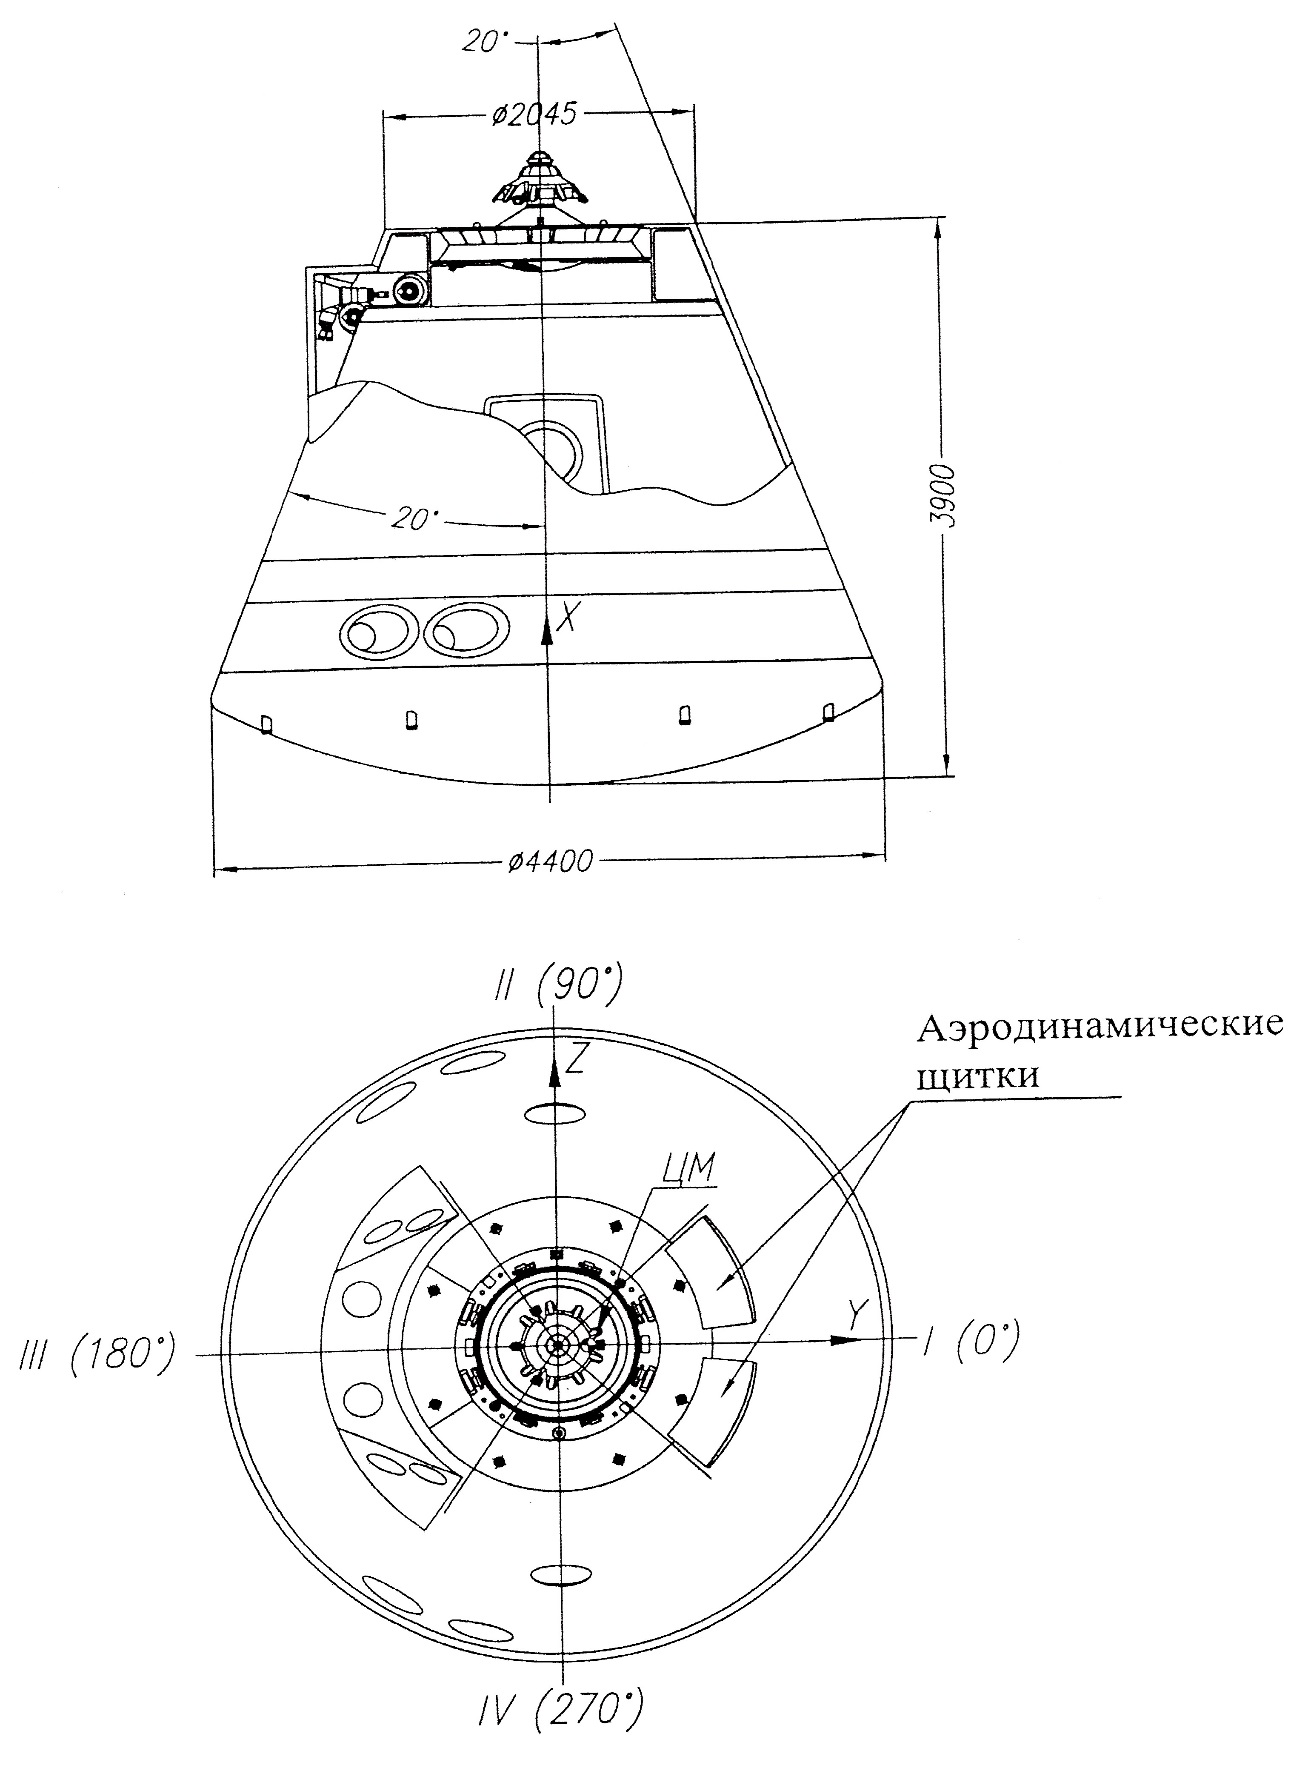
\includegraphics[scale=0.7]{images/va.jpg}
	\caption{Общий вид ВА}
	\label{fig:va_pic}
\end{figure}
\clearpage

\begin{figure}[h]
	\centering
	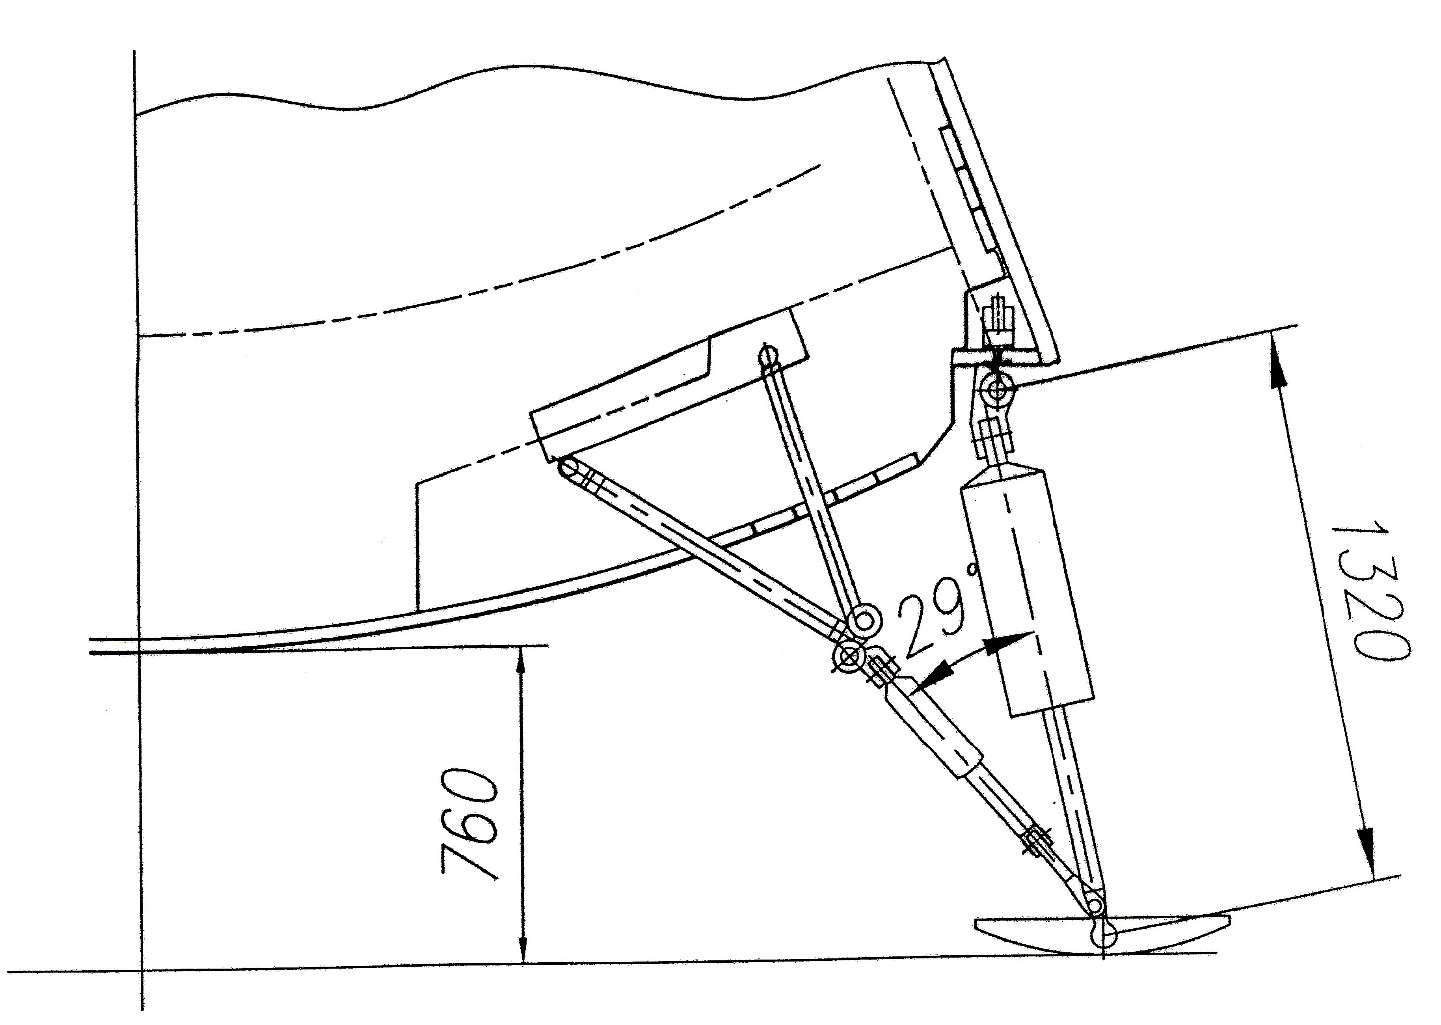
\includegraphics[scale=0.9]{images/posad_config.jpg}
	\caption{Посадочная конфигурация ВА с выпущенным посадочным устройством}
	\label{fig:posad_config}
\end{figure}
\clearpage

\subsection{Конструкция и принцип действия ПТДУ}
ПТДУ представляет собой РДТТ с регулируемой тягой по величине и направлению. На рисунке показана схема ПТДУ. Он состоит из:
\begin{itemize}
	\item двух корпусов типа "кокон"  с наполнителями ТРТ "Г-З"
	\item 16 односопловых управляющих блоков (СУБ)
	\item системы газоходов, газосвязывающего корпуса с наполнителями и СУБ
	\item двух пусковых двигателей 
	\item блока датчиков давления системы измерения давления
	\item рулевого привода (электромеханического или газогидравлического) 
\end{itemize}

Сопла всех СУБ снабжены собственными регуляторами расхода, управляемыми собственными рулевыми машинками. Расположение и маркировка органов управления соответствует рисунку 6.1.

ПТДУ многорежимна. Переход с режима на режим, а также стабилизация давления на любом режиме, обеспечивается изменением газоприхода от поверхности горения за счет изменения скорости горения наполнителя путем кратковременного изменения суммарной площади минимальных сечений сопел.

Создание управляющих сил по каналам тангажа и рыскания на каждом режиме обеспечивается за счет перераспределения расхода продуктов сгорания ТРТ между соплами путем изменения площади минимального сечения каждого сопла при сохранении постоянной суммарной площади минимальных сечений всех сопел:
\begin{equation}
\mu F_{\sum} = \sum_{j=1}^{16} \mu F_j \approx const
\end{equation}
где $\mu F_{\sum}$ - требуемая суммарная эффективная площадь минимальных сечений сопел на соответствующем режиме работы ПТДУ.

$\mu F_j$ - текущая эффективная площадь минимального сечения $j$-го сопла.

При необходимости должна быть обеспечена возможность отсечки тяги ПТДУ по команде СУ. При этом для прекращения горения наполнителей должно выполняться условие:
\begin{equation}
\mu F_{\sum} = \sum_{j=1}^{16} \mu F_j^{max}
\end{equation}
где $\mu F_j^{max}$ - максимальная эффективная площадь минимального сечения $j$ - го сопла.

В случае отказа одного из СУБ или отказа ПМ площадь минимального сечения этого СУБ при дальнешей работе ПТДУ должна оставаться постоянной, при это должна выполняться заданная циклограмма суммарной тяги $R_{\sum}$  и управление остальными СУБ в заданном диапазоне $R$.
\begin{figure}[h]
	\centering
	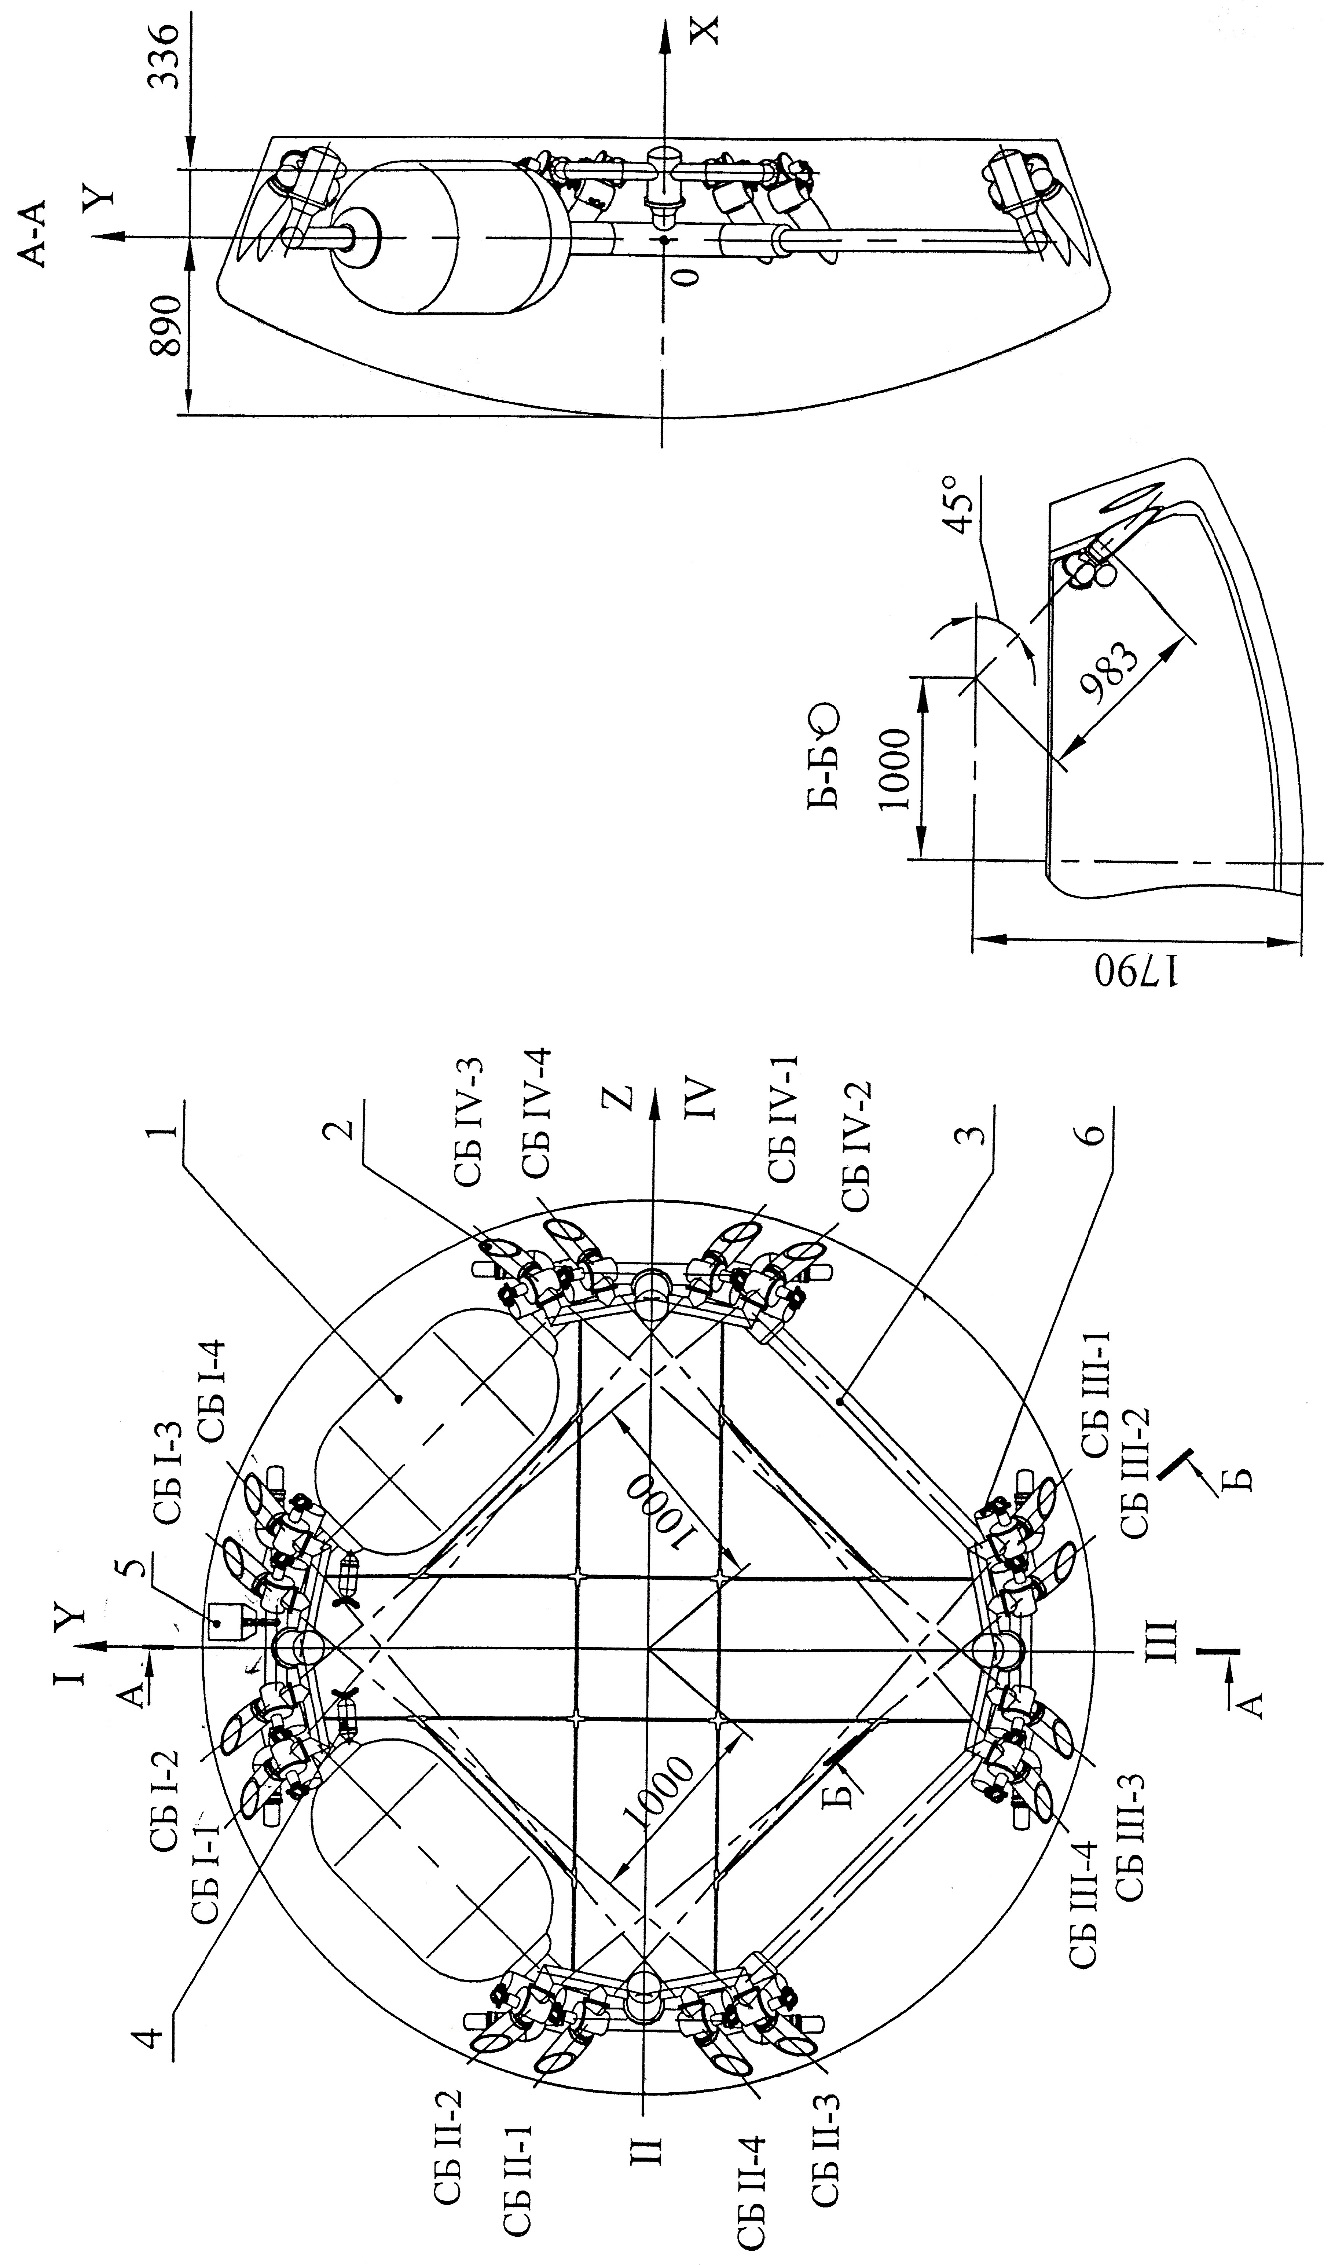
\includegraphics[scale=0.5, angle=-90]{images/scheme_ptdu.jpg}
	\caption{Схема ПТДУ}
	\label{fig:scheme_ptdu}
\end{figure}
\clearpage

\subsection{Характеристики органов управления}

\begin{figure}[h]
	\centering
	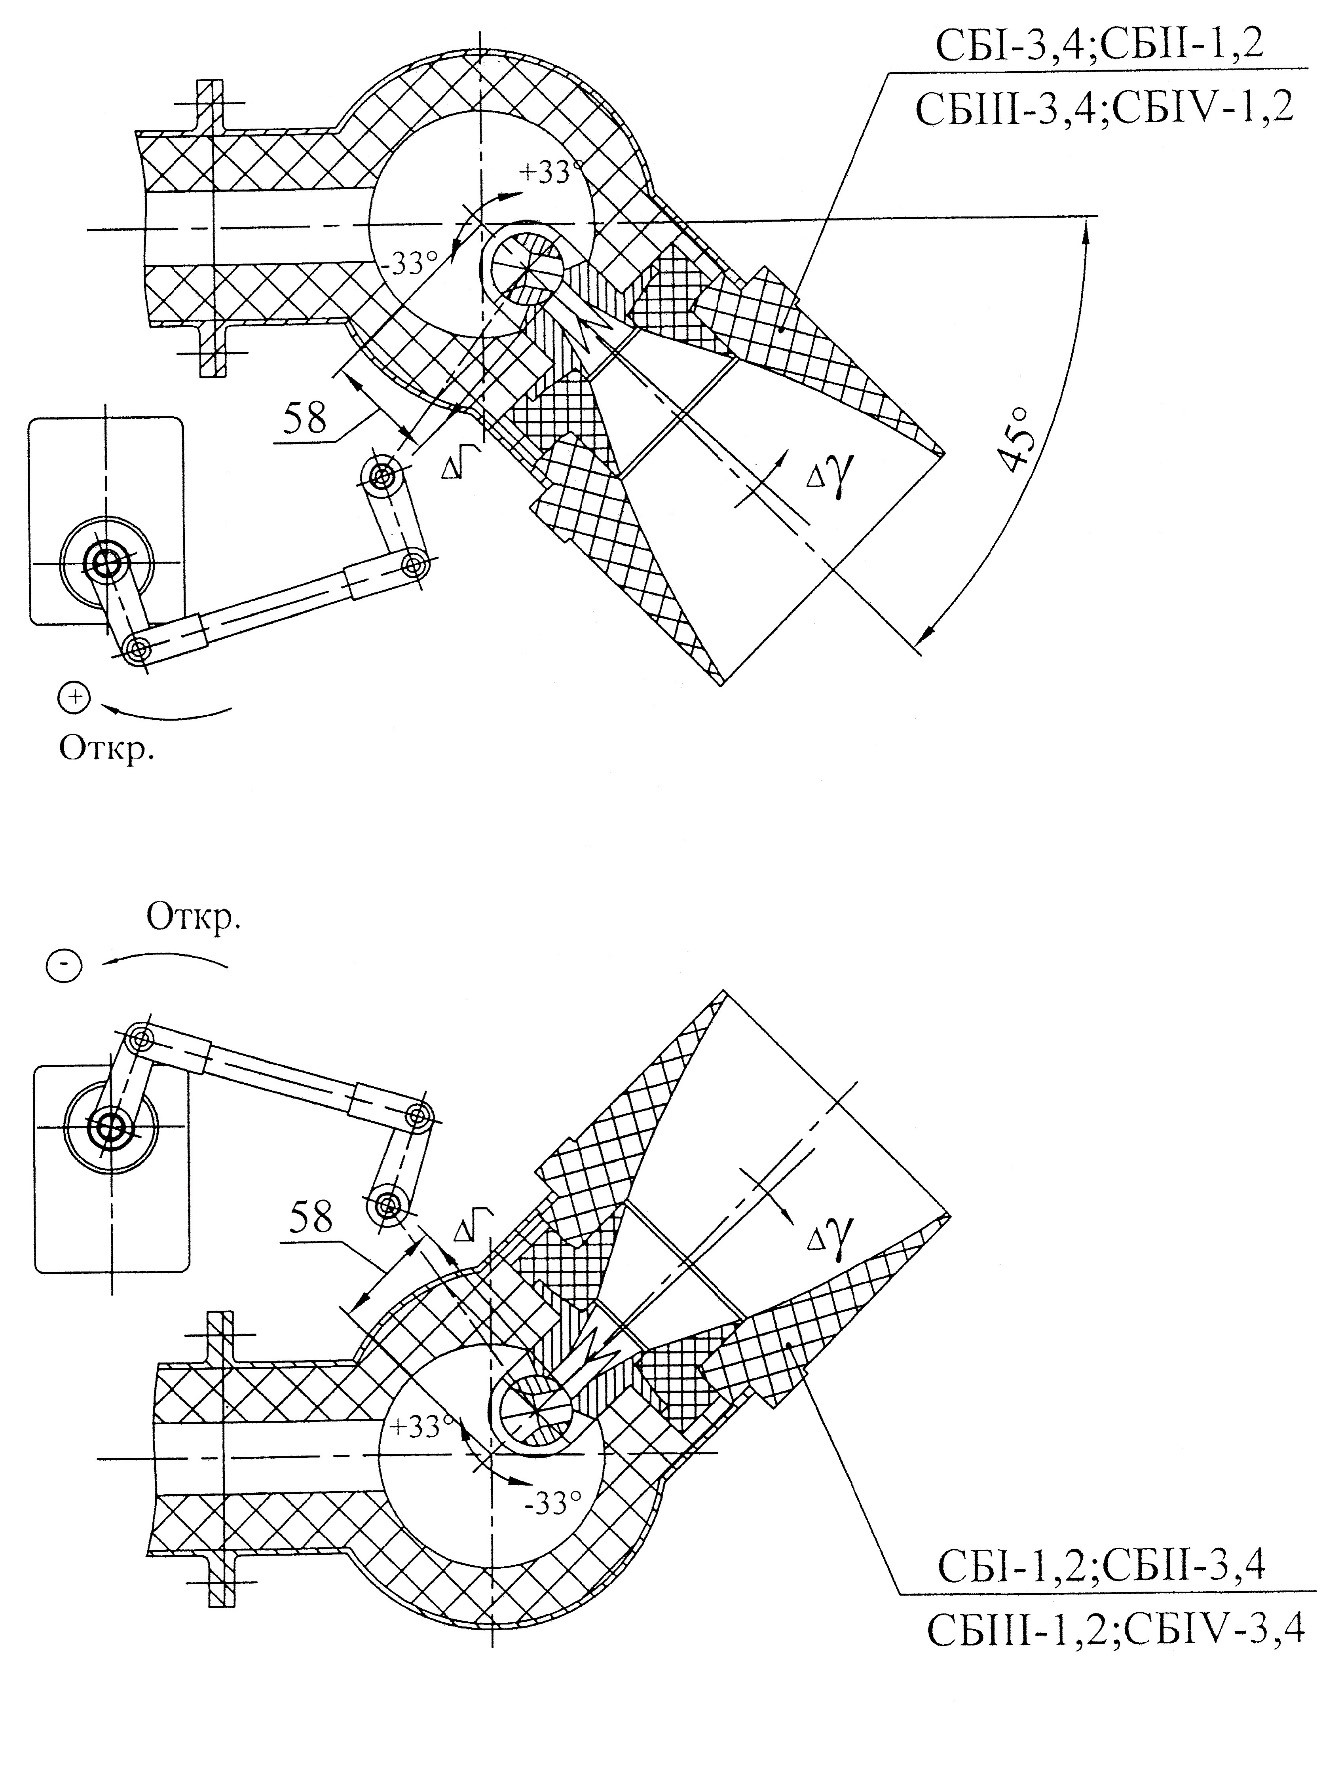
\includegraphics[scale=0.5]{images/scheme_subrp.jpg}
	\caption{Кинематическая схема СУБ с РП}
	\label{fig:scheme_subrp}
\end{figure}

Зависимость эффективной площади минимального сечения единичного сопла СУБ ($\mu F_j$) от угла поворота вала РМ ($\delta_j$ ) представлена на рисунке ~(\ref{fig:effect_nozzle})

\begin{figure}[h]
	\centering
	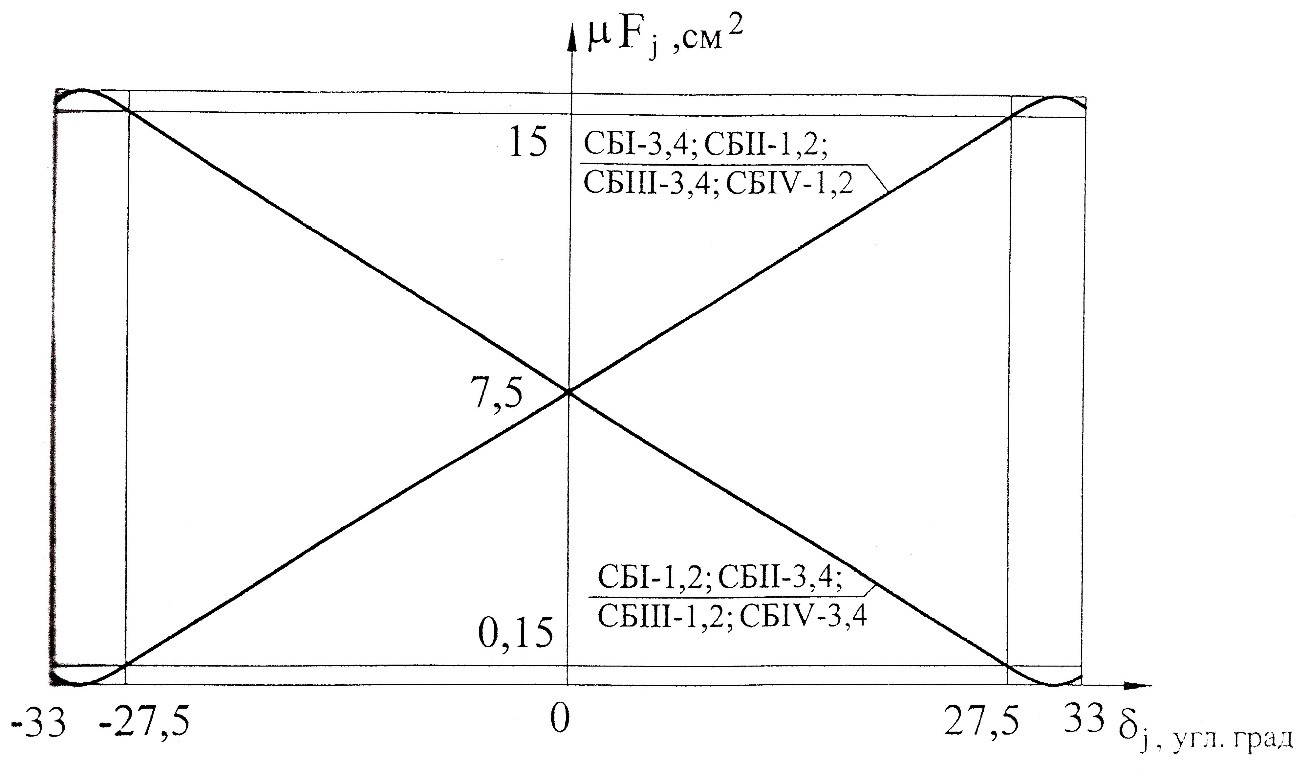
\includegraphics[scale=0.5]{images/effect_nozzle.jpg}
	\caption{Зависимость эффективной площади сечения единичного сопла ($\mu F_j$) от угла поворота вала РМ ($\delta_j$)}
	\label{fig:effect_nozzle}
\end{figure}

При работе ПТДУ используется только линейный участок зависимости $\mu F_j (\delta_j)$.

На участке от $-27.5^{\circ}$ до $27.5^{\circ}$ для данной расходной характеристики допускается линейная аппроксимация:
\begin{equation}
	\label{eq:ur_lin_approxim}
	\delta_j = 3.667 \cdot \mu F_j - 27.5
\end{equation}

Систематическое линейное и угловое отклонение вектора тяги в единичном сопле в зависимости от угла поворота РМ от геометрической оси сопла за счет прямоугольной формы площади минимального сечения регулятора сопла приведено на ~(\ref{fig:effect_nozzle}).

Отклонение происходит в плоскости, проходящей через геометрическую ось сопла перпендикулярно продольной оси корпуса СУБ.

Случайное отклонение вектора тяги от номинального положения геометрической оси сопла в плоскости минимального сечения составляет: линейное $1.5$ мм, угловое $1.5^{\circ}$.

\begin{figure}[h]
	\centering
	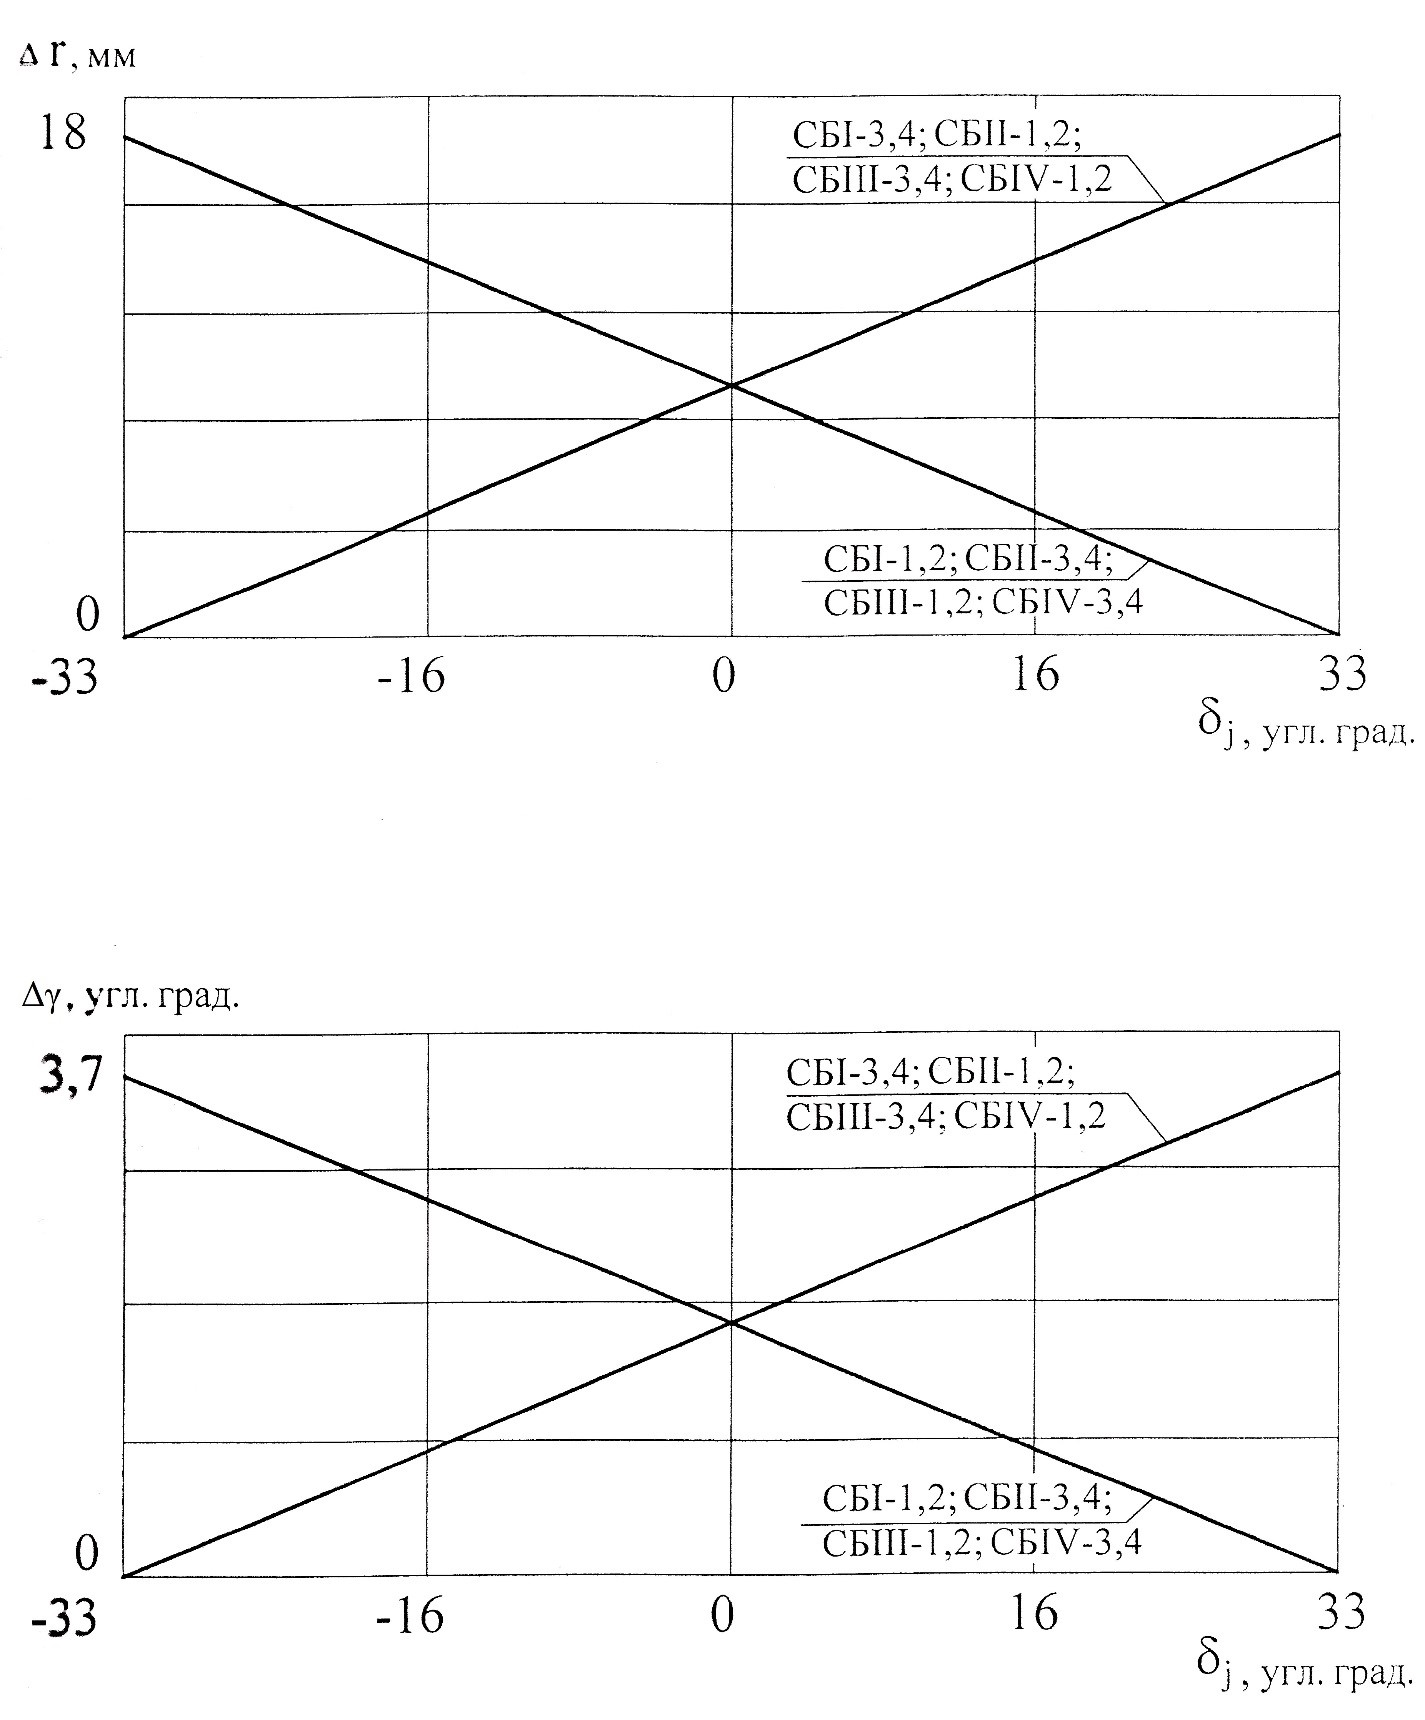
\includegraphics[scale=0.5]{images/linear_vect_draft.jpg}
	\caption{Линейное ($\Delta r$) и угловое ($\Delta \gamma$) отклонение линии действия вектора тяги от геометрической оси сопла в зависимости от угла поворота вала РМ}
	\label{fig:lin_angle_otklonenie}
\end{figure}

\clearpage

\subsection{Требования к СУ}
Исходными данными на разработку технических предложений по алгоритмам СУ, СУ ПТДУ для управления на участке посадки возвращаемого аппарата определены следующие положения:
\begin{itemize}
	\item Начальные условия при запуске ПТДУ:
	\begin{itemize}
		\item угол наклона траектории $-70^{\circ} \div -90^{\circ}$
		\item скорость $80 \div 120 \frac{\text{м}}{\text{с}}$
		\item угол атаки $8^{\circ} \div 20^{\circ} $
		\item угловые скорости до $\pm 50$ угл. град/с по трем углам одновременно
		\item высота $700 \div 1200$ м.
	\end{itemize}
	\item Условия окончания:
	\begin{itemize}
		\item на высоте ~ $20$ м начинается участок вертикального движения, который завершается касанием. Скорость во время касания $2 \div 3 \frac{\text{м}}{\text{с}}$
	\end{itemize}
	\item суммарный импульс тяги:
	$$\int \limits_{0}^T R(r) dt = 2745862 \ \text{Н} \cdot c$$
	\item Ограничения на СУ в вертикальном канале ВА:
	\begin{itemize}
		\item отклонение от требуемой траектория $\pm 5 \text{м}$
	\end{itemize}
\end{itemize}
\clearpage